\documentclass{article}
\usepackage[utf8]{inputenc}
\usepackage{tikz}
\usetikzlibrary{positioning}
\usetikzlibrary{shapes}

\begin{document}

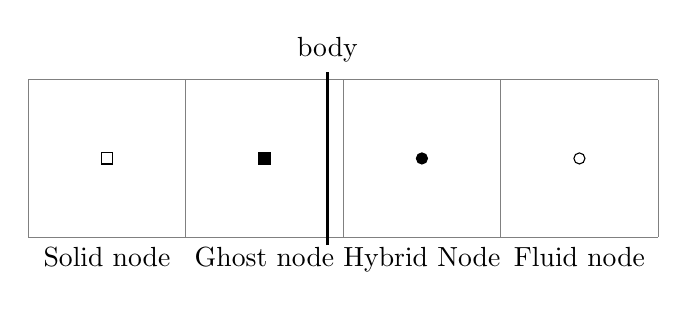
\begin{tikzpicture}
%grid
%horizontal
\draw[gray, thin] (-4,1) -- (4,1);
\draw[gray, thin] (-4,-1) -- (4,-1);
%vertical
\draw[gray, thin] (-4,1) -- (-4,-1);
\draw[gray, thin] (-2,1) -- (-2,-1);
\draw[gray, thin] (0,1) -- (0,-1);
\draw[gray, thin] (2,1) -- (2,-1);
\draw[gray, thin] (4,1) -- (4,-1);
%body
\draw[black, thick] (-0.2,-1.1) -- (-0.2,1.1) node[anchor=south] {body}; 
%nodes
\draw [black] (3.0,0) circle (2pt); %fluid
\draw ([xshift=-2pt,yshift=-2pt]-3.0,0) rectangle ++(4pt,4pt);%solid
\filldraw ([xshift=-2pt,yshift=-2pt]-1.0,0) rectangle ++(4pt,4pt);%ghost
\filldraw [black] (1,0) circle (2pt);%hybrid

%legend
\node[anchor=north] at (3.0,-1) {Fluid node};
\node[anchor=north] at (-3.0,-1) {Solid node};
\node[anchor=north] at (-1.0,-1) {Ghost node};
\node[anchor=north] at (1,-1.0) {Hybrid Node};

\end{tikzpicture}


\end{document}
